%!TEX root =main.tex
\section{Upper bounding the expressive power}
We start by assessing the expressive power of GNNs of the form~(\ref{eq:architecture}) in terms of vertex classification.
It is easy to see that GNNs of the form~(\ref{eq:architecture}) are not always bounded by WL, according to 
Definition~\ref{def:wlupper}. This should not come as a surprise since these architectures do not always fit in the general
GNN architecture~(\ref{lab:generalGNN}), for which boundedness by WL is guaranteed (by Proposition~\ref{prop:upperboundgeneral}).
Indeed, the update rules in~(\ref{eq:architecture})  have more information available in each step, in the form of the matrices $\mathbf{L}$ and $\mathbf{R}$, than the WL process. In terms of the general GNNs architecture~(\ref{lab:generalGNN}), the presence of $\mathbf{L}$ and $\mathbf{R}$ may require the combination and aggregation functions to be dependent on the \textit{vertex} under consideration. By contrast, these functions only depend on the \textit{features} of the vertex and its neighbors in the general GNN architecture~(\ref{lab:generalGNN}). We illustrate this with the following two examples.

\begin{example}\label{ex1}\normalfont
Consider the graph $G$ with two vertices $v$ and $w$ and a single (undirected) edge $\{v,w\}$. Let $\pmb{\ell}_v=\pmb{\ell}_w:=a$ and consider  $\mathbf{F}^{(0)}:=\left[\begin{smallmatrix}1\\1\end{smallmatrix}\right]$, $\mathbf{L}:=\mathbf{I}$,
 $\mathbf{R}:=\left[\begin{smallmatrix}1 & 0\\0& 2\end{smallmatrix}\right]$, $p=q:=0$ and $\mathbf{W}^{(0)}:=1$.
% Note that $\mathbf{F}^{(0)}\not\sqsubseteq \mathbf{R}$, so
% the conditions~(\ref{eq:conditions}) are not satisfied.
Then, according to the update rule~(\ref{eq:architecture}):
$$
\mathbf{F}^{(1)}:=\sigma\left(\mathbf{A}\mathbf{R}\mathbf{F}^{(0)}\mathbf{W}^{(0)}\right)=
\sigma\left(\begin{bmatrix}
0& 1 \\
1 & 0\\
\end{bmatrix}\begin{bmatrix}1 & 0\\0& 2\end{bmatrix}\begin{bmatrix}1\\1\end{bmatrix}\right)=\begin{bmatrix}\sigma(2)\\\sigma(1)\end{bmatrix}.
$$
Let 
$\pmb{\ell}^{(0)}:=\pmb{\ell}$.
It is now readily verified that $\pmb{\ell}^{(t)}_v=\pmb{\ell}^{(t)}_w$ for all $t\geq 0$. So, WL will classify both vertices as the same. We further note that  $\pmb{\ell}^{(0)}\equiv \mathbf{F}^{(0)}$. Nevertheless, $\pmb{\ell}^{(1)}\not\sqsubseteq \mathbf{F}^{(1)}$ whenever $\sigma(2)\neq\sigma(1)$. This happens, for example, when $\sigma$ is the ReLU activation function. Hence, the architecture is not bounded by WL. Similar examples can be constructed using the matrix $\mathbf{L}$  and for other choices of the activation function $\sigma$. \qed
\end{example}

A less artificial example is based on the NA-GNN+ architecture~\cite{kipf-loose}.

\begin{example}\label{ex2}\normalfont
Consider the labeled graph $(G,\pmb{\ell})$ (\raisebox{-2ex}{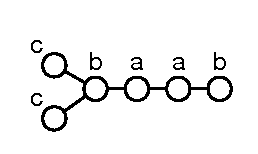
\includegraphics[height=1cm]{graph1}}) with 
vertex labeling  $\pmb{\ell}_{v_1}=\pmb{\ell}_{v_2}=c$,
$\pmb{\ell}_{v_3}=\pmb{\ell}_{v_6}=b$ and $\pmb{\ell}_{v_4}=\pmb{\ell}_{v_5}=a$, and adjacency and degree matrix 
$$
\mathbf{A}:=\begin{bmatrix}
0 & 0 & 1 & 0 & 0 & 0\\
0 & 0 & 1 & 0 & 0 & 0\\
1 & 1 & 0 & 1 & 0 & 0\\
0 & 0 & 1 & 0 & 1 & 0\\
0 & 0 & 0 & 1 & 0 & 1\\
0 & 0 & 0 & 0 & 1 & 0
\end{bmatrix}\text{ and } 
\mathbf{D}:=
\begin{bmatrix}
1 & 0 & 0 & 0 & 0 & 0\\
0 & 1 & 0 & 0 & 0 & 0\\
0 & 0 & 3 & 0 & 0 & 0\\
0 & 0 & 0 & 2 & 0 & 0\\
0 & 0 & 0 & 0 & 2 & 0\\
0 & 0 & 0 & 0 & 0 & 1
\end{bmatrix},
$$
respectively. 
We consider $\mathbf{F}^{(1)}:=\sigma(\tilde{\mathbf{D}}^{-1/2}(\mathbf{A}+\mathbf{I})\tilde{\mathbf{D}}^{-1/2}\mathbf{F}^{(0)}\mathbf{W}^{(0)})$ with  $
\mathbf{F}^{(0)}=
\left[\begin{smallmatrix}
1 & 0 & 0\\
1 & 0 & 0\\
0 & 1 & 0\\
0 & 0 & 1\\
0 & 0 & 1\\
0 & 1 & 0\\
\end{smallmatrix}\right]
$ and choose $\mathbf{W}^{(0)}=\left[\begin{smallmatrix}
1 & 0 & 0\\
0 & 1 & 0\\
0 & 0 & 1
\end{smallmatrix}\right]$. 
We remark that $\pmb{\ell}^{(0)}:=\pmb{\ell}\equiv \mathbf{F}^{(0)}$.
It can be verified that
$$
\mathbf{F}^{(1)}=\sigma\left(\begin{bmatrix}
\frac{1}{2} & \frac{1}{2\sqrt{2}}& 0\\
\frac{1}{2} & \frac{1}{2\sqrt{2}}& 0\\
\frac{1}{2\sqrt{2}} & \frac{1}{4}& \frac{1}{
2\sqrt{3}}\\
0 & \frac{1}{2\sqrt{3}}& \frac{2}{
3}\\
0 & \frac{1}{\sqrt{6}}& \frac{2}{
3}\\
0 & \frac{1}{2}& \frac{1}{
\sqrt{6}}
\end{bmatrix}\right).
$$
Suppose that $\sigma$ is the ReLU activation function. Then, we observe that
$\mathbf{F}^{(1)}_{v_4\bullet}\neq \mathbf{F}^{(1)}_{v_5\bullet}$. 
We note, however, that $\pmb{\ell}^{(1)}_{v_4}=(a,\{a,b\})=\pmb{\ell}^{(1)}_{v_5}$.
Hence, $\pmb{\ell}^{(1)}\not\sqsubseteq \mathbf{F}^{(1)}$ and this architecture is not bounded by WL.
\openprob{Is there a simple example for the one below?}
\qed
% It can, however, be verified that $\pmb{\ell}^{(2)}\sqsubseteq \mathbf{F}^{(1)}$.
% \todo{The latter inclusion needs to be verified}\qed
\end{example}
We will next provide an upper bound for  GNN architectures of the form~(\ref{eq:architecture}) by revising the labeling used in the graph.


\subsection{A general bound}\label{subsec:generalupb}
As we have seen above, for a fair comparison with GNNs of the form~(\ref{eq:architecture}), the WL process needs to have access to the information in the $\mathbf{L}$ and $\mathbf{R}$ matrices. To this aim we extend the set $\Sigma$ of labels.
Let  $(G,\pmb{\ell})$ be a labeled graph and assume that $\pmb{\ell}:V\to \Sigma$. Given $\mathbf{L}$, $\mathbf{R}$  we define $L:=\{ \mathbf{L}_{vv} \mid v\in V\}$ and
$R:=\{ \mathbf{R}_{vv} \mid v\in V\}$.
We define the set $\hat \Sigma$ of \textit{extended labels} as $\hat \Sigma:=\Sigma \cup \Sigma\times L\times R$. Given $(G,\pmb{\ell})$, we consider labeled graph $(G,\hat{\pmb{\ell}})$ with labeling
$$
\hat{\pmb{\ell}}_v:=\langle \pmb{\ell}_v, \mathbf{L}_{vv},\mathbf{R}_{vv}\rangle,
$$
for $v\in V$.
We can now bound the expressive power of  GNN architecture of the form~(\ref{eq:architecture}) by WL \textit{provided that we use the extended labels}. As before, we denote by 
$\hat{\pmb{\ell}}{}^{(t)}$ the labeling obtain after $t$ steps of the WL algorithm on $(G,\hat{\pmb{\ell}})$, starting from $\hat{\pmb{\ell}}{}^{(0)}:=\hat{\pmb{\ell}}$.

\begin{theorem}\label{thm:generalbound}
Let $(G,\pmb{\ell})$ be a labeled graph and assume that $\pmb{\ell}\sqsubseteq\mathbf{F}^{(0)}$.
Then, GNN architectures of the form~(\ref{eq:architecture}) are bounded by WL on $(G,\hat{\pmb{\ell}})$.
\end{theorem}
\begin{proof}
We show the upper bound by WL by induction on the number of iterations. For $t=0$, we have, by assumption, that 
$\pmb{\ell}\sqsubseteq \mathbf{F}^{(0)}$. Clearly,
$\hat{\pmb{\ell}}{}^{(0)}\sqsubseteq \pmb{\ell}$ and hence also 
$\hat{\pmb{\ell}}{}^{(0)}\sqsubseteq\mathbf{F}^{(0)}$. We next assume that the induction hypothesis holds for $t\geq 0$ and consider $t+1$. We need to show that 
$\hat{\pmb{\ell}}{}^{(t+1)}_v=\hat{\pmb{\ell}}{}^{(t+1)}_w$ implies that $\mathbf{F}^{(t+1)}_{v\bullet}=\mathbf{F}^{(t+1)}_{w\bullet}$. By definition,
$\hat{\pmb{\ell}}{}^{(t+1)}_v=\hat{\pmb{\ell}}{}^{(t+1)}_w$ implies
$\hat{\pmb{\ell}}{}^{(t)}_v=\hat{\pmb{\ell}}{}^{(t)}_w$ and 
$$
\ldbl \hat{\pmb{\ell}}{}^{(t)}_u \st u \in N_G(v) \rdbl=
 \ldbl \hat{\pmb{\ell}}{}^{(t)}_u \st u \in N_G(w) \rdbl.$$
 Since $\hat{\pmb{\ell}}{}^{(t)}\sqsubseteq \hat{\pmb{\ell}}{}^{(t-1)}\sqsubseteq \cdots\sqsubseteq \hat{\pmb{\ell}}{}^{(0)}$, this implies that
 $\hat{\pmb{\ell}}{}^{(0)}_v=\hat{\pmb{\ell}}{}^{(0)}_w$ and that there is a bijection $b:N_G(v)\to N_G(w):u\mapsto u'$ such that $\hat{\pmb{\ell}}{}^{(t)}_u=\hat{\pmb{\ell}}{}^{(t)}_{u'}$ and hence also 
 $\hat{\pmb{\ell}}{}^{(0)}_u=\hat{\pmb{\ell}}{}^{(0)}_{u'}$. From the definition of $\hat{\pmb{\ell}}{}^{(0)}$, $\hat{\pmb{\ell}}{}^{(0)}_v=\hat{\pmb{\ell}}{}^{(0)}_w$ implies that
 $\mathbf{L}_{vv}=\mathbf{L}_{ww}$ and
 $\mathbf{R}_{vv}=\mathbf{R}_{ww}$. Similarly, for every $u\in N_G(v)$ and corresponding $u'\in N_G(w)$,
$\hat{\pmb{\ell}}{}^{(0)}_u=\hat{\pmb{\ell}}{}^{(0)}_{u'}$ implies that   $\mathbf{L}_{uu}=\mathbf{L}_{u'u'}$ and $\mathbf{R}_{uu}=\mathbf{R}_{u'u'}$. By the induction hypothesis we also have that
 $\mathbf{F}^{(t)}_{v\bullet}=\mathbf{F}^{(t)}_{w\bullet}$, and for every $u\in N_G(v)$
   and corresponding $u'\in N_G(w)$, $\mathbf{F}^{(t)}_{u\bullet}=\mathbf{F}^{(t)}_{u'\bullet}$. It now suffices to observe that
  \begin{align*}
	  \mathbf{F}^{(t+1)}_{v\bullet}&=\sigma\Biggl(\mathbf{F}^{(t-1)}_{v\bullet}\mathbf{W}_1^{(t-1)}+\mathbf{L}_{vv}\biggl(\Bigl(\sum_{u\in N_G(v)} \mathbf{R}_{uu}\mathbf{F}^{(t)}_{u\bullet}\Bigr)+p\mathbf{R}_{vv}\mathbf{F}^{(t)}_{v\bullet}\biggr)\mathbf{W}^{(t)}+ q\mathbf{J}_{v\bullet}\Biggr)\\
	 & =\sigma\Biggl(\mathbf{F}^{(t-1)}_{w\bullet}\mathbf{W}_1^{(t-1)}+\mathbf{L}_{ww}\biggl(\Bigl(\!\!\sum_{u'\in N_G(w)}\!\! \mathbf{R}_{u'u'}\mathbf{F}^{(t)}_{u'\bullet}\Bigr)+p\mathbf{R}_{ww}\mathbf{F}^{(t)}_{w\bullet}\biggr)\mathbf{W}^{(t)}+ q\mathbf{J}_{w\bullet}\Biggr)\\
	  &=\mathbf{F}^{(t+1)}_{w\bullet},
\end{align*}
as desired.
\end{proof}

\begin{example}\label{ex3}\normalfont
	Continuing with Example~\ref{ex1}, $\hat{\pmb{\ell}}_v:=\langle a,1,1\rangle$ and $\hat{\pmb{\ell}}_w:=\langle a,1,2\rangle$. Hence, $\hat{\pmb{\ell}}{}^{(1)}_v:=(\langle a,1,1\rangle,\{\langle a,1,2\rangle\})$ and $\hat{\pmb{\ell}}{}^{(1)}_w:=(\langle a,1,2\rangle,\{\langle a,1,1\rangle\})$ and $v$ and $w$ are labeled differently in the first step of WL, starting from $\hat{\pmb{\ell}}{}^{(0)}:=\hat{\pmb{\ell}}$. Clearly,
	$\hat{\pmb{\ell}}{}^{(1)}\sqsubseteq \mathbf{F}^{(1)}$ with $\mathbf{F}^{(1)}=\left[\begin{smallmatrix}\sigma(2)\\\sigma(1)\end{smallmatrix}\right]$.
	Continuing with Example~\ref{ex2}, 
$\hat{\pmb{\ell}}_{v_1}=\hat{\pmb{\ell}}_{v_1}:=\langle c, \frac{1}{\sqrt{2}},\frac{1}{\sqrt{2}}\rangle$,
 $\hat{\pmb{\ell}}_{v_3}=\langle b, \frac{1}{\sqrt{4}},\frac{1}{\sqrt{4}}\rangle$, $\hat{\pmb{\ell}}_{v_4}=\hat{\pmb{\ell}}_{v_5}=\langle a, \frac{1}{\sqrt{3}},\frac{1}{\sqrt{3}}\rangle$, and $\hat{\pmb{\ell}}_{v_6}=\langle b,\frac{1}{\sqrt{2}},\frac{1}{\sqrt{2}}\rangle$. Hence, whereas $\pmb{\ell}^{(1)}_{v_4}=\pmb{\ell}^{(1)}_{v_5}$ we now have that
$$
\hat{\pmb{\ell}}{}^{(1)}_{v_4}:=(\langle a, \frac{1}{\sqrt{3}},\frac{1}{\sqrt{3}}\rangle,\{
\langle a, \frac{1}{\sqrt{3}},\frac{1}{\sqrt{3}}\rangle,\langle b, \frac{1}{\sqrt{4}},\frac{1}{\sqrt{4}}\rangle\})
\neq
\hat{\pmb{\ell}}{}^{(1)}_{v_5}:=(\langle a, \frac{1}{\sqrt{3}},\frac{1}{\sqrt{3}}\rangle,\{
\langle a, \frac{1}{\sqrt{3}},\frac{1}{\sqrt{3}}\rangle,\langle b, \frac{1}{\sqrt{2}},\frac{1}{\sqrt{2}}\rangle\}).
$$	It can be verified that $\hat{\pmb{\ell}}{}^{(1)}\sqsubseteq \mathbf{F}^{(1)}$.
	\qed
\end{example}

We will complement Theorem~\ref{thm:generalbound}  with the corresponding lower bound in Section~\ref{sec:lowerb}. In fact, we verify the lower bound already for a slightly simpler class of GNNs than those of the form~(\ref{eq:architecture}).
\floris{It seems that we need lower bounds for two classes (see next section.) So this may need to be revised.}
\begin{theorem}\label{thm:lowerb_general}
The class of GNNs of the form 
\begin{equation}
\mathbf{F}^{(t)}:=\sigma\left(\mathbf{L}(\mathbf{A}+p\mathbf{I})\mathbf{R}\mathbf{F}^{(t-1)}\mathbf{W}^{(t-1)} + q\mathbf{J}\right), \label{eq:architecture_lb}
\end{equation}
is WL-strong, where WL now starts from $(G,\hat{\pmb{\ell}})$. Here, $\sigma$ can be either the sign or the ReLU activation function.
\end{theorem}
This class of GNNs differs from GNNs of the form~(\ref{eq:architecture}) by eliminating  the weight matrices $\mathbf{W}_1^{(t)}$.


\subsection{Special cases}\label{subsec:specialcases}
We next observe that in some cases one can still bound  GNNs of the form~(\ref{eq:architecture}) in terms of WL using the given labeling $\pmb{\ell}$ instead of
$\hat{\pmb{\ell}}$ on $G$. 

% A trivial case for which this holds are adjacency GNNs:
% \begin{description}
%  \item[\textit{Adjacency} (A-GNN):]
% % $\mathbf{L}=\mathbf{R}:=\mathbf{I}$, $p=q:=0$. Hence,
% $
% \mathbf{F}^{(t)}:=\sigma\left(\mathbf{A}\mathbf{F}^{(t-1)}\mathbf{W}^{(t)}\right).
% $
% \end{description}
%
% Indeed, if we consider the adjacency architecture then
% $\hat{\pmb{\ell}}_v:=\langle \pmb{\ell}_v,1,1\rangle$ and thus $\hat{\pmb{\ell}}\equiv\pmb{\ell}$. In this case, the architecture will be bounded by 1-WL
% in the usual way, i.e., starting from $\pmb{\ell}^{(0)}:=\pmb{\ell}$. This holds more generally.
For example, consider GNNs of the form~\ref{eq:groheGNNwithJ}. Here, we have that $\mathbf{L}=\mathbf{R}=\mathbf{I}$. As consequence, for any labeled graph $(G,\pmb{\ell})$
we have that  $\hat{\pmb{\ell}}_v:=\langle \pmb{\ell}_v,1,1\rangle$ and thus $\hat{\pmb{\ell}}\equiv\pmb{\ell}$. In this case, the GNN will be bounded by 1-WL in the usual way, i.e., starting from $\pmb{\ell}^{(0)}:=\pmb{\ell}$. 

\begin{corollary}\label{cor:adjacency}
GNNs of the form~(\ref{eq:architecture}) for which 
$\pmb{\ell}\sqsubseteq\hat{\pmb{\ell}}$ holds, for any labeled graph $(G,\pmb{\ell})$, are bounded by WL, starting from $\pmb{\ell}^{(0)}:=\pmb{\ell}$. 
% In particular, the adjacency architecture is bounded by 1-WL.
\end{corollary}
\begin{proof}
For any labeled graph $(G,\pmb{\ell})$ we always have that $\hat{\pmb{\ell}}\sqsubseteq \pmb{\ell}$. Hence, the assumption $\pmb{\ell}\sqsubseteq\hat{\pmb{\ell}}$ implies that $\pmb{\ell}\equiv\hat{\pmb{\ell}}$. As a consequence, $\pmb{\ell}^{(t)}\equiv \hat{\pmb{\ell}}{}^{(t)}$ for all $t\geq 0$. Theorem~\ref{thm:generalbound} then implies $\hat{\pmb{\ell}}{}^{(t)}\sqsubseteq \mathbf{F}^{(t)}$, and hence also $\pmb{\ell}^{(t)}\sqsubseteq\mathbf{F}^{(t)}$.
\end{proof}
Intuitively, if $\pmb{\ell}\sqsubseteq\hat{\pmb{\ell}}$ holds for any labeled graph $(G,\pmb{\ell})$, then this implies that the matrices $\mathbf{L}$ and $\mathbf{R}$ must
be constant. Indeed, just consider the uniform labeling $\pmb{\ell}_v:=a$ for all $v\in V$. Then,
$\pmb{\ell}\equiv\hat{\pmb{\ell}}$ if and only if $\mathbf{L}_{vv}=\mathbf{L}_{ww}$
and $\mathbf{R}_{vv}=\mathbf{R}_{ww}$ for all vertices.
This is clearly the case for GNNs of the form~(\ref{eq:groheGNNwithJ}).
Another way of verifying Corollary~\ref{cor:adjacency} is that when $\mathbf{L}$ and $\mathbf{R}$ are constant, then GNNs of the form
~(\ref{eq:architecture}) can be seen as GNN of the form~\ref{lab:generalGNN}, and Proposition~\ref{prop:upperboundgeneral} applies.

In view of Corollary~\ref{cor:adjacency}, we remark that Theorem~\ref{thm:lowerb_general} implies that when $\mathbf{L}$ and $\mathbf{R}$ are constant matrices, the corresponding class of GNNs is WL-strong, starting from $(G,\pmb{\ell})$. This holds in particular
for the class of GNNs of the form~\ref{eq:groheGNNwithJ}. Hence, we recover the result from~\cite{grohewl} stating that GNNs of the form~\ref{eq:groheGNNwithJ} are WL-strong. Furthermore, as anticipated, the lower bound also holds for the ReLU function. We defer the details of the lower bounds to Section~\ref{sec:lowerb}.

As a second example, consider a NA-GNN+. For those GNNs, we have that $\mathbf{L}_{vv}=\frac{1}{\sqrt{1+d_v}}$
and $\mathbf{R}_{vv}=\frac{1}{\sqrt{1+d_v}}$. This implies that
for any labeled graph $(G,\pmb{\ell})$ we have that $\pmb{\ell}^{(1)}\sqsubseteq\hat{\pmb{\ell}}$
holds. Indeed, if $\pmb{\ell}^{(1)}_v=\pmb{\ell}^{(1)}_w$ then $\pmb{\ell}_v=\pmb{\ell}_w$ and for every $u\in N_G(v)$ and corresponding $u'\in N_G(w)$,
$\pmb{\ell}_u=\pmb{\ell}_{u'}$. In particular, $d_{v}=d_w$ and thus  $\pmb{\ell}^{(1)}\sqsubseteq\hat{\pmb{\ell}}$. More generally, if $\pmb{\ell}^{(1)}\sqsubseteq\hat{\pmb{\ell}}$ holds for any labeled graph $(G,\pmb{\ell})$,
then the entries of $\mathbf{L}$ and $\mathbf{R}$ must be functionally determined by the
degrees of the vertices. To see this, it suffices to consider again the uniform labeling
$\pmb{\ell}_v:=a$ for all $v\in V$. Then, $\pmb{\ell}^{(1)}\sqsubseteq\hat{\pmb{\ell}}$ implies that
for any two vertices $v$ and $w$, 
$$(a,\underbrace{\ldbl a, a,\ldots, a\rdbl}_{|N_G(v)|=d_v})=
(a,\underbrace{\ldbl a, a,\ldots, a\rdbl}_{|N_G(w)|=d_w}),$$
or in other words, $d_v=d_w$. So, when  $d_v=d_w$ we have $\hat{\pmb{\ell}}_v=\hat{\pmb{\ell}}_w$, or $d_v=d_w$ implies $\mathbf{L}_{vv}=\mathbf{L}_{ww}$ and $\mathbf{R}_{vv}=\mathbf{R}_{ww}$.

\begin{corollary}\label{cor:augmented2}
GNNs of the form~(\ref{eq:architecture}) for which 
$\pmb{\ell}^{(1)}\sqsubseteq\hat{\pmb{\ell}}$ holds, for any labeled graph $(G,\pmb{\ell})$, are bounded by WL, starting from $\pmb{\ell}^{(1)}$. 
\end{corollary}
\begin{proof}
If 	$\pmb{\ell}^{(1)}\sqsubseteq\hat{\pmb{\ell}}$ holds, then also 
$\pmb{\ell}^{(t+1)}\sqsubseteq\hat{\pmb{\ell}}{}^{(t)}$ holds for any $t\geq 0$. Hence,
$\pmb{\ell}^{(t+1)}\sqsubseteq \mathbf{F}^{(t)}$ 
% or $\pmb{\ell}^{(1)}\sqsubseteq\mathbf{F}^{(t-1)}$ by
by Theorem~\ref{thm:generalbound}.
\end{proof}

This upper bound holds for all special GNNs listed at the end of the previous section. Indeed,
Indeed, $\hat{\pmb{\ell}}_v:=\langle \pmb{\ell}_v,1,1\rangle$ for GNNs of the form ~(\ref{eq:groheGNNwithJ}),
$\hat{\pmb{\ell}}_v:=\langle \pmb{\ell}_v,1/d_{v},1\rangle$ for RW-GNNS,
$\hat{\pmb{\ell}}_v:=\langle \pmb{\ell}_v,1/\sqrt{d_{v}},1/\sqrt{d_{v}}\rangle$ for NA-GNNs,1-GCN's and 1-GCNs's, 
$\hat{\pmb{\ell}}_v:=\langle \pmb{\ell}_v,1/\sqrt{1+d_{v}},1\rangle$ for RW-GNN+
$\hat{\pmb{\ell}}_v:=\langle \pmb{\ell}_v,1/\sqrt{1+d_{v}},1/\sqrt{1+d_{v}}\rangle$ for NA-GNN+, as we have seen already above, and 
$\hat{\pmb{\ell}}_v:=\langle \pmb{\ell}_v,1/\sqrt{r+(1-r)d_{v}},1/\sqrt{r+(1-r)d_{v}}\rangle$ 
for NA-GNN++.

We note than when a GNN is bounded by WL, starting from $\pmb{\ell}^{(k)}$, it is also bounded by WL, starting from $\pmb{\ell}^{(k')}$ for all $k'\geq k$. The converse is not necessarily true, as is illustrated by the following example for NA-GNN+'s.
\begin{example}\label{ex4}\normalfont
Going back to  Example~\ref{ex2}, we know from Corollary~\ref{cor:augmented2} that NA-GNN+'s are bounded WL, starting from $\pmb{\ell}^{(1)}$. It can indeed be verified that in Example~\ref{ex2}, $\pmb{\ell}^{(2)}\sqsubseteq \mathbf{F}^{(1)}$. We have seen, however, that $\pmb{\ell}^{(1)}\not\sqsubseteq \mathbf{F}^{(1)}$. Hence, NA-GNN+'s are not necessarily bounded by WL, starting from $\pmb{\ell}^{(0)}$.\qed
\end{example}
It can also be verified that the previous example works for 1-GCNs's (and thus also for 1-GCN's) and NA-GNN's (and thus also NA-GNN++'s).
\begin{example}\normalfont
	Using the same setting as in Example~\ref{ex2}, it can be verified that 
	$$\mathbf{F}^{(1)}=\sigma\left(\begin{bmatrix}
	1 & 1/6 & 0\\
	1 & 1/6 & 0\\
	1/3 & 1 & 1/6\\
	0 & 1/6 & 5/4\\
	0 & 1/2 & 5/4\\
    0 & 1 & 1/2	\end{bmatrix}\right) \text{ and }
 \mathbf{F}^{(1)}=\sigma\left(\begin{bmatrix}
	0 & 1/6 & 0\\
	0 & 1/6 & 0\\
	1/3 & 0 & 1/6\\
	0 & 1/6 & 1/4\\
	0 & 1/2 & 1/4\\
    0 & 0 & 1/2	\end{bmatrix}\right), $$
	for 1-GCNs and for NA-GNNs, respectively. In both case, we see that $\pmb{\ell}^{(1)}\not\sqsubseteq \mathbf{F}^{(1)}$. Hence, these architectures are not necessarily bounded by WL, starting from $\pmb{\ell}$.\qed
\end{example}


We will complement Corollary~\ref{cor:augmented2} by the following lower bound in Section~\ref{sec:lowerb}.
\floris{Again, we need two such results, in order to capture all our GNN architectures. See next section.}

\begin{theorem}
GNNs of the form~(\ref{eq:architecture}) for which 
$\pmb{\ell}^{(1)}\sqsubseteq\hat{\pmb{\ell}}$ holds, for any labeled graph $(G,\pmb{\ell})$, are WL-strong, starting from $\pmb{\ell}^{(1)}$. 
\end{theorem}
In particular, we show this lower bound holds already for GNNs of the form~(\ref{eq:architecture_lb})
for which $\pmb{\ell}^{(1)}\sqsubseteq\hat{\pmb{\ell}}$ holds, for any labeled graph $(G,\pmb{\ell})$.



% Corollary~\ref{cor:augmented} applies for $k=1$ for the random walk, normalized adjacency, augmented random walk and augmented adjacency architectures. Indeed, for these architectures,
% $\hat{\pmb{\ell}}_v:=\langle \pmb{\ell}_v,1/d_{v},1\rangle$,
% $\hat{\pmb{\ell}}_v:=\langle \pmb{\ell}_v,1/\sqrt{d_{v}},1/\sqrt{d_{v}}\rangle$,
% $\hat{\pmb{\ell}}_v:=\langle \pmb{\ell}_v,1/\sqrt{1+d_{v}},1\rangle$, and
% $\hat{\pmb{\ell}}_v:=\langle \pmb{\ell}_v,1/\sqrt{(1+d_{v})},1/\sqrt{(1+d_{v}})\rangle$, respectively. For none of these architecture the inclusion $\pmb{\ell}\sqsubseteq \hat{\pmb{\ell}}$ necessarily holds. We note, however, that when $\pmb{\ell}^{(1)}_v=\pmb{\ell}^{(1)}_w$ then $\pmb{\ell}_v=\pmb{\ell}_w$ and for every $u\in N_G(v)$ and corresponding $u'\in N_G(w)$,
% $\pmb{\ell}_u=\pmb{\ell}_{u'}$. In particular, $d_{v}=d_w$. Hence, $\pmb{\ell}^{(1)}\sqsubseteq\hat{\pmb{\ell}}$. As a consequence,  Corollary~\ref{cor:augmented} implies:
% \begin{corollary}\label{cor:augmented2}
% The random walk, normalized adjacency, augmented random walk and augmented adjacency architectures are  bounded by 1-WL, starting from $\pmb{\ell}^{1}$.
% \end{corollary}


A careful look at the  proof of Theorem~\ref{thm:generalbound} reveals that
the roles of $\mathbf{L}$ and $\mathbf{R}$ in the GNN architectures~(\ref{eq:architecture})
are different. Indeed, if we wish to compute the feature vector $\mathbf{F}^{(t+1)}_{v\bullet}$ of a vertex $v$, then only $\mathbf{L}_{vv}$
is required from $\mathbf{L}$. By contrast, we need  $\mathbf{R}_{vv}$ and $\mathbf{R}_{uu}$ for every $u\in N_G(v)$ from $\mathbf{R}$. As it turns out,
even when $\hat{\pmb{\ell}}\not\equiv \pmb{\ell}$, it is sometimes the case that the architecture is still bounded by WL, starting from $\pmb{\ell}$. 

For example, if we take any of the GNNs for which $\mathbf{L}$ is functionally determined by
the degrees of vertices and for which $\mathbf{R}=\mathbf{I}$, then for any labeled graph $(G,\pmb{\ell})$ we have that $\pmb{\ell}^{(1)}\sqsubseteq \hat{\pmb{\ell}}$ holds, as before. In addition, however, we have that $\pmb{\ell}_v=\pmb{\ell}_w\Rightarrow \mathbf{R}_{vv}=\mathbf{R}_{ww}$. It is easy to see that this condition  corresponds to 
$\mathbf{L}$ being functionally determined by degree information, and $\mathbf{R}$ being a constant matrix. We remark that these conditions are satisfied for RW-GNNs and RW-GNN+'s
and GNNs of the form~\ref{eq:groheGNNwithJ}. 

\begin{corollary}\label{cor:weak}
	GNNs of the form~(\ref{eq:architecture}) for which 
	$\pmb{\ell}^{(1)}\sqsubseteq\hat{\pmb{\ell}}$  and
	$\pmb{\ell}^{(0)}_v=\pmb{\ell}^{(0)}_w\Rightarrow \mathbf{R}_{vv}=\mathbf{R}_{ww}$ hold,
 for any labeled graph $(G,\pmb{\ell})$, are bounded by WL, starting from $\pmb{\ell}$.
% For any $k'<k$ such that $\pmb{\ell}^{(k)}\sqsubseteq \hat{\pmb{\ell}}$ and
% $\pmb{\ell}^{(k')}_v=\pmb{\ell}^{(k')}_w\Rightarrow \mathbf{R}_{vv}=\mathbf{R}_{ww}$ hold, we have that GNN architectures of the form~(\ref{eq:architecture})  are bounded by 1-WL, starting from $\pmb{\ell}^{(k-1)}$.
\end{corollary}
\begin{proof}
We need to show that $\pmb{\ell}^{(t)}_v=\pmb{\ell}^{(t)}_w$ implies $\mathbf{F}^{(t)}_{v\bullet}=\mathbf{F}^{(t)}_{w\bullet}$ for $t\geq 0$.
We show this by induction on $t$. For $t=0$, we have by assumption that $\pmb{\ell}^{(0)}\sqsubseteq \mathbf{F}^{(0)}$.
 % and since $\pmb{\ell}^{(k-1)}\sqsubseteq\pmb{\ell}^{(0)}$ also $\pmb{\ell}^{(k-1)}\sqsubseteq\mathbf{F}^{(0)}$.
 Consider $t\geq 1$ and assume that $\pmb{\ell}^{(t)}_v=\pmb{\ell}^{(t)}_w$. This implies that $\pmb{\ell}^{(t-1)}_v=\pmb{\ell}^{(t-1)}_w$ and for every $u\in N_G(v)$ and corresponding $u'\in N_G(w)$, $\pmb{\ell}^{(t-1)}_u=\pmb{\ell}^{(t-1)}_{u'}$.
By induction, $\mathbf{F}^{(t-1)}_{v\bullet}=\mathbf{F}^{(t-1)}_{w\bullet}$ and for every $u\in N_G(v)$ and corresponding $u'\in N_G(w)$,  $\mathbf{F}^{(t-1)}_{u\bullet}=\mathbf{F}^{(t-1)}_{u'\bullet}$. 
We observe that $\pmb{\ell}^{(t)}_v=\pmb{\ell}^{(t)}_w$ implies that
$\pmb{\ell}^{(1)}_v=\pmb{\ell}^{(1)}_w$ since $t\geq 1$.
Hence,
% $\pmb{\ell}^{(1)}\sqsubseteq \hat{\pmb{\ell}}$ for $t\geq k$. Hence,
$\mathbf{L}_{vv}=\mathbf{L}_{ww}$ and $\mathbf{R}_{vv}=\mathbf{R}_{ww}$. Furthermore, 
$\pmb{\ell}^{(t-1)}_u=\pmb{\ell}^{(t-1)}_{u'}$ does not necessary implies that 
$\pmb{\ell}^{(1)}_v=\pmb{\ell}^{(1)}_w$ (e.g., when $t=1$). It does, however imply that
$\pmb{\ell}_u=\pmb{\ell}_{u'}$ and hence, by assumption, $\mathbf{R}_{uu}=\mathbf{R}_{u'u'}$. 
Hence, also $\pmb{\ell}^{(t-1)}_u=\pmb{\ell}^{(t-1)}_{u'}\Rightarrow \mathbf{R}_{uu}=\mathbf{R}_{u'u'}$.
Hence,
$\pmb{\ell}^{(t-1)}_u=\pmb{\ell}^{(t-1)}_{u'}$ implies $\mathbf{R}_{uu}=\mathbf{R}_{u'u'}$ for every $u\in N_G(v)$ and corresponding $u'\in N_G(w)$.
This suffices to conclude that 
  \begin{align*}
	  \mathbf{F}^{(t)}_{v\bullet}&=\sigma\Biggl(\mathbf{F}^{(t-1)}_{u\bullet}\mathbf{W}_1^{(t-1)}+\mathbf{L}_{vv}\biggl(\Bigl(\sum_{u\in N_G(v)} \mathbf{R}_{uu}\mathbf{F}^{(t-1)}_{u\bullet}\Bigr)+p\mathbf{R}_{vv}\mathbf{F}^{(t-k)}_{v\bullet}\biggr)\mathbf{W}^{(t-1)}+ q\mathbf{J}_{v\bullet}\Biggr)\\
	 & =\sigma\Biggl(\mathbf{F}^{(t-1)}_{v\bullet}\mathbf{W}_1^{(t-1)}+\mathbf{L}_{ww}\biggl(\Bigl(\!\!\sum_{u'\in N_G(w)}\!\! \mathbf{R}_{u'u'}\mathbf{F}^{(t-1)}_{u'\bullet}\Bigr)+p\mathbf{R}_{ww}\mathbf{F}^{(t-1)}_{w\bullet}\biggr)\mathbf{W}^{(t-1)}+ q\mathbf{J}_{w\bullet}\Biggr)\\
	  &=\mathbf{F}^{(t)}_{w\bullet},
\end{align*}
as desired.
\end{proof}

We will  show in the next section that GNNs of the form~(\ref{eq:architecture}) for which 
$\pmb{\ell}^{(1)}\sqsubseteq\hat{\pmb{\ell}}$  and 
	$\pmb{\ell}^{(0)}_v=\pmb{\ell}^{(0)}_w\Rightarrow \mathbf{R}_{vv}=\mathbf{R}_{ww}$ hold,
 for any labeled graph $(G,\pmb{\ell})$, are also WL-strong,  starting from $\pmb{\ell}$.
 
 

%
%
%
% %
% % As we will see shortly, this holds for the random walk and augmented random walk architectures.
% % % We start by identifying conditions on
% % $\hat{\pmb{\ell}}$ that result in the architecture to be only $k-1$ steps ahead of $1$-WL, rather than $k$-steps ahead as reported in Corollary~\ref{cor:augmented}.
%
% \begin{corollary}\label{cor:weak}
% For any $k'<k$ such that $\pmb{\ell}^{(k)}\sqsubseteq \hat{\pmb{\ell}}$ and
% $\pmb{\ell}^{(k')}_v=\pmb{\ell}^{(k')}_w\Rightarrow \mathbf{R}_{vv}=\mathbf{R}_{ww}$ hold, we have that GNN architectures of the form~(\ref{eq:architecture})  are bounded by 1-WL, starting from $\pmb{\ell}^{(k-1)}$.
% \end{corollary}
% We remark that the assumptions on  $\pmb{\ell}$ and $\hat{\pmb{\ell}}$ are satisfied for the
% random walk and augmented random walk architectures. Indeed, for these architectures,
% $\hat{\pmb{\ell}}_v:=\langle \pmb{\ell}_v,1/d_{v},1\rangle$ and
% $\hat{\pmb{\ell}}_v:=\langle \pmb{\ell}_v,1/\sqrt{1+d_{v}},1\rangle$, respectively. We have seen before that
% $\pmb{\ell}^{(1)}\sqsubseteq \hat{\pmb{\ell}}$. Moreover, $\pmb{\ell}^{(0)}_v=\pmb{\ell}^{(0)}_w$ implies
% $\mathbf{R}_{vv}=1=\mathbf{R}_{ww}$. Hence, Corollary~\ref{cor:weak}, for $k=1$ and $k'=0$, implies:
%
% \begin{corollary}\label{cor:augrw1wl}
% The random walk and augmented random walk architectures are bounded by 1-WL, starting from $\pmb{\ell}^{(0)}$.
% \end{corollary}
%
% It remains to show Corollary~\ref{cor:weak}. The proof is minor modification of the proof of Theorem~\ref{thm:generalbound}.


\floris{Not sure whether we want the following. It is just a generalization which basically says that if you put $k$-WL related stuff in $\mathbf{L}$ and $\mathbf{R}$ you are bounded by $\pmb{\ell}^{(k)}$. Let's discuss whether we want this. }
We conclude this section by observing that Corollaries~\ref{cor:augmented2} and~\ref{cor:weak} generalize as follows. 
\begin{corollary}\phantom{This is just a dummy line}
\begin{itemize}
\item[(a)] GNNs of the form~(\ref{eq:architecture}) for which 
	$\pmb{\ell}^{(k)}\sqsubseteq\hat{\pmb{\ell}}$  holds,
 for any labeled graph $(G,\pmb{\ell})$, are bounded by WL, starting from $\pmb{\ell}^{(k)}$.
\item[(b)] GNNs of the form~(\ref{eq:architecture}) for which 
	$\pmb{\ell}^{(k)}\sqsubseteq\hat{\pmb{\ell}}$  and
	$\pmb{\ell}^{(k')}_v=\pmb{\ell}^{(0)}_w\Rightarrow \mathbf{R}_{vv}=\mathbf{R}_{ww}$ with $k'<k$ hold,
 for any labeled graph $(G,\pmb{\ell})$, are bounded by WL, starting from $\pmb{\ell}^{(k-1)}$.
\end{itemize}	
\end{corollary}
%  $\pmb{\ell}^{(k)}\sqsubseteq\hat{\pmb{\ell}}$
% and $\pmb{\ell}^{(k)}\sqsubseteq\hat{\pmb{\ell}}$ and $$
%
% Remark: iterated degrees...
% More generally, we have the following property.
% \begin{corollary}\label{cor:augmented}
% If $\pmb{\ell}^{(k)}\sqsubseteq\hat{\pmb{\ell}}$ holds, then the GNN architecture~(\ref{eq:architecture})  is bounded by 1-WL, starting from $\pmb{\ell}^{(k)}$.
% \end{corollary}
% Intuitively, this implies that the GNN architecture is $k$-steps ahead of the 1-WL algorithm.
% More precisely, $\pmb{\ell}^{(t)}\sqsubseteq \mathbf{F}^{(t-k)}$ for $t\geq k$.
\begin{proof}
	For (a)~, if 	$\pmb{\ell}^{(k)}\sqsubseteq\hat{\pmb{\ell}}$ holds, then also 
$\pmb{\ell}^{(k+t)}\sqsubseteq\hat{\pmb{\ell}}{}^{(t)}$ holds for any $t\geq 0$. Hence,
$\pmb{\ell}^{(k+t)}\sqsubseteq \mathbf{F}^{(t)}$ or $\pmb{\ell}^{(k)}\sqsubseteq\mathbf{F}^{(t-k)}$ by Theorem~\ref{thm:generalbound}.
For (b)~, it is easily verified that the proof of Corollary~\ref{cor:weak} can be generalized to this setting.
\end{proof}
Intuitively, when $\pmb{\ell}^{(k)}\sqsubseteq\hat{\pmb{\ell}}$ holds for any labeled graph $(G,\pmb{\ell})$, then this implies that the entries in $\mathbf{L}$ and $\mathbf{R}$ are functionally determined by the so-called \textit{$k$-iterated degrees} of vertices. The $k$-iterated degree of a vertex $v$ is the label assigned by $k$-steps of  WL on the uniformily labeled graph $(G,\pmb{a})$ in which every vertex is assigned the label $a$.
Similarly, $\pmb{\ell}^{(k')}_v=\pmb{\ell}^{(0)}_w\Rightarrow \mathbf{R}_{vv}=\mathbf{R}_{ww}$ implies that the entries in $\mathbf{R}$ are functionally determined by the $k'$-iterated degrees of vertices. We illustrate this by the following example.
\begin{example}
	\floris{Show example for say, $k=2$, and $k=2$ and $k'=1$, if we think this is interesting.}
\end{example}
